%% Template for ENG 401 reports
%% by Robin Turner
%% Adapted from the IEEE peer review template

%
% note that the "draftcls" or "draftclsnofoot", not "draft", option
% should be used if it is desired that the figures are to be displayed in
% draft mode.

\documentclass[peerreview]{IEEEtran}
\usepackage{cite} % Tidies up citation numbers.
\usepackage{url} % Provides better formatting of URLs.
\usepackage[utf8]{inputenc} % Allows Turkish characters.
\usepackage{booktabs} % Allows the use of \toprule, \midrule and \bottomrule in tables for horizontal lines
\usepackage{graphicx}
\usepackage{amssymb}
\usepackage{amsmath}
\usepackage{breqn}

\hyphenation{op-tical net-works semi-conduc-tor ThaumatoAnakalyptor} % Corrects some bad hyphenation 



\begin{document}
%\begin{titlepage}
% paper title
% can use linebreaks \\ within to get better formatting as desired
\title{ThaumatoAnakalyptor \\ Technical Report and Roadmap}


% author names and affiliations

\author{Julian Schilliger \\
Vesuvius Challenge\\
}
\date{February 19, 2024}

% make the title area
\maketitle
\tableofcontents
\listoffigures
\listoftables
%\end{titlepage}

\IEEEpeerreviewmaketitle
\begin{abstract}
ThaumatoAnakalyptor \cite{thaumato} is the first advanced automatic segmentation pipeline designed for high-precision extraction of papyrus sheet segmentations from Computed Tomography (CT) scans of ancient scrolls with minimal human intervention. The pipeline has multiple steps. First, a 3D PointCloud extraction step extracts points laying on the papyrus surfaces from the 3D CT scroll scan. 3D Instance Segmentation extracts smaller PointCloud sheet patches from the scroll surface PointCloud. These sheet patches are overlapping each other and are combined to a sheet surface segmentation using a Random Walk stitching procedure. Poisson Surface Reconstruction generates a surface mesh from the segmentation. Flattened UV coordinates are added to the surface mesh by utilizing a cylindrical unrolling and flattening with the help of SLIM. Finally, the mesh is rendered into a tiff surface volume.

\end{abstract}





\section{Introduction}
Segmenting the Herculaneum Papyri is a difficult task because of the damaged nature of the scrolls and the tightly wound papyrus. Multiple wraps of papyrus can be fused together, ripped, partially missing or strongly deformed. Inspecting the 3D CT scroll scans by eye shows how difficult it is even for humans to correctly attribute different sections of the papyrus to the appropriate windings.

% An example of a floating figure using the graphicx package.
% Note that \label must occur AFTER (or within) \caption.
% For figures, \caption should occur after the \includegraphics.
% Note that IEEEtran v1.7 and later has special internal code that
% is designed to preserve the operation of \label within \caption
% even when the captionsoff option is in effect. However, because
% of issues like this, it may be the safest practice to put all your
% \label just after \caption rather than within \caption{}.
%
% Reminder: the "draftcls" or "draftclsnofoot", not "draft", class
% option should be used if it is desired that the figures are to be
% displayed while in draft mode.
%
\begin{figure}[!h]
\centering
\includegraphics[width=0.8\columnwidth]{scroll1} 
\caption{Slice through Scroll 1}
\label{fig_sim}
\end{figure}

% Note that IEEE typically puts floats only at the top, even when this
% results in a large percentage of a column being occupied by floats.


\section{Problem Definition}
Segmentation in the area of Virtual Restoration of ancient scrolls describes the process of extracting the papyrus sheet's surface from a CT scan of the rolled-up scroll.

\section{Segmentation Pipeline}
ThaumatoAnakalyptor is a pipeline that has as input the CT scanned scroll in the format of a stack of 2D tiff images. The output is a 3D mesh containing the flattened UV coordinates of each mesh vertex.
In this section, I describe all the different pipeline steps, their data input and output and the algorithms working on the data.

\subsubsection{Volume Coordinate System}
The 3D CT volume has indexes $X$, $Y$, $Z$. The 2D tiff stack has for each 2D tiff picture the coordinates $X$, $Y$ in direct mapping and $Z$ as the index of the 2D tiff image.

\subsubsection{Pipeline Overview}
This is the flow of the data:
\begin{itemize}
    \item Scroll Data
    \item Grid Cells
    \item Papyrus Surface PointCloud
    \item Surface Patches PointClouds
    \item Patches Stitching
    \item Mesh Reconstruction
    \item Mesh Flattening
    \item Surface Volume Texturing
    \item Ink Detection
\end{itemize}



\subsection{Scroll Data}
The pipeline expects the scroll scan as a 2D tiff image stack. Each 2D image has single channeled pixels of datatype uint16. Based on this volume, the center of the scroll in 3D is extracted into an "umbilicus.txt" file.
Each entry in the umbilicus file is in the format $Y + 500$, $Z + 500$, $X + 500$. The entries are sorted from lowest to highest $Z$ value. The complete umbilicus (center of the scroll) for every $Z$ value is generated by interpolating linearly between each two adjacent data points.

\subsection{2D Tiff Stack to 3D Tiff "Grid Cells"}
Since ThaumatoAnakalyptor works in 3D, the data is first transformed into a more suitable data format for faster access during computation.
The 2D tiff stack is used to build 3D tiff files of size 500x500x500 voxels spanning the entire volume. These are called Grid Cells. All Grid Cells are the same size. They index the $X,Y$ coordinates from the 2D tiffs and the numbering $Z$ of the 2D tiffs as follows: grid\_cell\_yxz\_\{X/500 + 1\}\_\{Y/500 + 1\}\_\{Z/500 + 1\}. Notable is the one-indexing. 

An example: grid\_cell\_yxz\_1\_1\_1 contains the Voxels from ($0$, $0$, $0$) to ($499$, $499$, $499$). This rule is true for all following volume formats.

\subsubsection{Code}
\begin{itemize}
    \item generate\_half\_sized\_grid.py
\end{itemize}

\subsection{Grid Cells to PointCloud}
\label{pointcloud}
The Grid Cells are then used to generate Surface Subvolumes PointClouds of size 200x200x200 voxels (Bug/Special "feature" note: size is actually 201 voxels each, but they are generated by a step size of 200 voxels), which in total are spanning the entire volume. The 200x200x200 sized input 3D image is padded by 50 voxels in each direction to ensure proper derivative calculation for the target PointCloud subvolume and the input data is extracted from the Grid Cells. In the region of these blocks, the 3D gradients in the corresponding 3D Grid Cell ares are analyzed with the first and second derivatives. The derivatives are normed to the general intensity of the voxels in the local area.

In detail, Thaumato first uniformly blurs the extracted 3D image with kernel size $11$ to remove high frequency noise. It then employs a Sobel filter in 3D to extract the Sobel vector $v_S^V$ ($\mathbb{R}^{3}$) for every voxel $V$ in the subvolume. The Sobel vectors are sub-sampled by stride $10$ in every dimension. By establishing the directionality of $v_S^V$ wrt. to the interpolated umbilicus point $P_y$ at the same height $y$, the vector is conditionally flipped to point in the general direction of $P_y$. To calculate an approximation of the local sheet normal $n_V$, the mean of all conditionally flipped vectors is calculated in a window of size $9$ in the sub-sampled volume and represents an estimate of the sheet normal in the vicinity of $V$. Trilinear interpolation is used to interpolate back to the pre-sampled volume. The vector  $v_S^V$ is then projected onto the vector $n_v$ and the norm with sign ($d_1^{'}$) is calculated. To ensure good generality of the derivatives for different scroll scans that have different mean intensities or different scroll areas with vastly different mean intensities, the derivatives $d_1$ of the subvolume are normed:
\[
d_1 = \frac{d_1^{'}}{\max (\max{d_1^{'}, ||\min d_1^{'}||})}
\]
This is used as the 1D first derivative $d_1$ in the sheet normal direction.

The First 1D derivatives in scroll direction then are used to calculate the second derivative in a similar manner. Sobel is applied to the first derivatives volume. The signed norm wrt. to the estimated sheet normal is calculated and results in $d_2^{'}$. $d_2^{'}$ is again normed like $d_1^{'}$ and results in $d_2$.

To extract the PointCloud, thresholding on $d_1$ and $d_2$ is employed with points fulfilling
\[
d_1 > 0.075
\]
and
\[
||d_2|| < 0.002
\].

All subvolumes together form the complete scroll surface PointCloud. The files are located in the folder "point\_cloud\_colorized\_verso". Note: The Verso and Recto naming is mixed up.
Definition of the PointCloud cell indexes $x'$, $y'$, $z'$:
\[
x' = (X + 500)/200
\]
\[
y' = (Y + 500)/200
\]
\[
z' = (Z + 500)/200
\]

The ".ply" files are indexed as follows: cell\_yxz\_\{x'\}\_\{y'\}\_\{z'\}. Each point in the resulting PointCloud represents a point that lies on the recto facing side of the rolled up papyrus sheets. To go from PointCloud coordinate system $x$, $y$, $z$ to scroll coordinate system $X$, $Y$, $Z$, note the position offset and axis swap:
\[
x = Y + 500
\]
\[
y = Z + 500
\]
\[
z = X + 500
\]

The PointClouds in the .ply files have an additional $color$ field for every point. These are 3 double values that are uniformly distributed in the range $0$ to $1$. Later on in the pipeline, they can be used to efficiently extract a subset of points from the PointCloud.

\subsubsection{Code}
\begin{itemize}
    \item grid\_to\_pointcloud.py
    \item surface\_detection.py
    \item add\_random\_colors\_to\_pointcloud.py
\end{itemize}

\subsection{PointCloud to Instances}
The PointCloud of the surface points is then used to extract single sheet PointClouds. Therefore the entire PointCloud is split into overlapping 200x200x200 sized blocks. The blocks are extracted with a step size of 100. The blocks are down-scaled to 50x50x50. Their coordinates are $x''$, $y''$, $z''$:

\[
x'' = x / 4
\]
\[
y'' = y / 4
\]
\[
z'' = z / 4
\]

Then this data is run trough a 3D instance segmentation model Mask3D\cite{mask3d} to extract the instances of each sheet PointCloud present in the subvolume. Mask3D predicts the top $25$ possible sheet instances of each patch. All sheet instances of the subvolume are then filtered to contain a minimum (parameterizeable) number of points and checked that the model assigned a reasonable (parametrizeable) certainty to the predicted sheet patches (.plys) and are then numbered starting from $0$ and saved together in a .tar file. The .tar files are located in the folder "point\_cloud\_colorized\_verso\_subvolume\_blocks". The .tars are indexed as $X''\_Y''\_Z''.tar$:

\[
X'' = prepend_6(x' / 4)
\]
\[
Y'' = prepend_6(y' / 4)
\]
\[
Z'' = prepend_6(z' / 4)
\]
With $prepend_6$ being a function that prepends the input to the length of $6$ positions with $0$'s.

\subsubsection{Code}
\begin{itemize}
    \item pointcloud\_to\_instances.py
    \item mask3D/inference.py
\end{itemize}

\subsection{Mask3D}
Mask3D \cite{mask3d} is used to generate the instance segmentation of the sheet patches. Training data is generated with two different methods.

Synthetic data is generated by incrementally adding planar surface patches to a volume, thereby varying the PointCloud density, the distance and planar angles. The volume is randomly distorted and rotated before cut into the appropriate dimensions.

Raw sample data from the pipeline step in subsection \ref{pointcloud} is annotated in CloudCompare. The different sheets are extracted. 

All the data is preprocessed into the right format for training Mask3D. Mask3D was trained for around $75$ epochs.

\subsubsection{Code}
\begin{itemize}
    \item generate\_surface\_pointgroup\_dataset.py
    \item generate\_training\_samples\_from\_annotations.py
    \item mask3D/inference.py
\end{itemize}


\subsection{Patches Stitching}
The Patches Stitching computation steps takes as input the segmented surface patches .tar files and a starting point in the scroll volume coordinate. It is unknown how many windings of the papyrus exist in the scroll.

The patch containing the point closest to the starting point is extracted and is the starting patch. The starting patch is added to the segmentation. 

The concept of the uncertainty graph used in the patches stitching process is defined as follows:

Let \(G = (V, E)\) be an undirected, weighted graph where:

\begin{itemize}
    \item \(V\) represents the set of nodes, each corresponding to a unique sheet patch \(patch^i_{a, b, c}\), extracted from the segmented surface patches. The indices \(a\), \(b\), and \(c\) denote the coordinates of the patch in the volume, and \(i\) is the identifier of the patch within its subvolume.
    \item \(E\) is the set of edges between nodes in \(V\). An edge exists between nodes \(u\) and \(v\) if and only if their similarity score is above a $thresh_{score}$ and the patches corresponding to \(u\) and \(v\) overlap according to:
    \[
    I_0 \cdot \lvert a_0-a_1 \rvert + I_1 \cdot \lvert b_0-b_1 \rvert + I_2 \cdot \lvert c_0-c_1 \rvert = 25
    \]
    holds, with \(I\in \{0, 1\}^3\) and \(||I|| = 1\). This is just the mathematical formulation of the meaning, that the patches are overlapping with 50\% overlap.
    
\end{itemize}

To compare overlapping patches, the degree of overlap in the pointcoulds is calculated. The weight of an edge \((u, v) \in E\) is determined by the similarity score between the two patches corresponding to \(u\) and \(v\), calculated as:

\[
similarity\ score = \\
\begin{cases}
    nrp\_factor \cdot score,& \text{if } score\geq 0 \\
    -1,             & \text{otherwise}
\end{cases}
\]

where

\begin{dmath}
nrp\_factor = \\
\begin{cases}
\log \left( \log \left( nrp \right) + 1 \right) + 1,& \text{if } ||patch_u \cap patch_v|| \geq thresh_{min} \\
    0,             & \text{otherwise}
\end{cases}
\end{dmath}

\begin{dmath}
    nrp = \\
    \frac{\min \left( \max \left(thresh_{min}, ||patch_u \cap patch_v||\right), thresh_{max} \right)}{thresh_{min}}
\end{dmath}

and

\begin{dmath}
    score =
\begin{cases}
    \left(\frac{overlap - thresh_{overlap}}{1 - thresh_{overlap}}\right)^2,& \text{if } overlap\geq tresh_{overlap} \\
    -1,              & \text{otherwise}
\end{cases}
\end{dmath}

with

\[
overlap = \frac{||patch_u \cap patch_v||}{\max (||patch_u||, ||patch_v||)},
\]

where \(||patch_u \cap patch_v||\) denotes the count of overlapping points between the two patches, \(thresh_{min}\) and \(thresh_{max}\) are parameters that define the range of acceptable overlaps for calculating \(nrp\), and \(thresh_{overlap}\) is a parameter that determines the minimum required overlap percentage for an edge to exist.

The graph \(G\) facilitates the identification of patches that are connected through the weighted edges. Usually $||V|| \geq 100'000$.

The task is to add a winding number $k_v \in \mathbb{R}$, that assigns each patch $v \in V$ to a winding in the scroll or determine that $v$ is noise and should be excluded from the sheet reconstruction. The winding number is calculated with the angle between the umbilicus and the patch centroid. The starting point has winding number $0$. 

Then the undirected, unweighted graphs \(G_{solution}\) can be constructed, that only contain nodes that are not noise and edges between patches, that are overlapping and where their winding number difference is smaller than an epsilon $0 < \epsilon \ll 1$.  We search \(G_{solution}^{*}\) such that $||E_{solution}^{*}||$ is maximal.


A custom Random Walk procedure then walks over the graph \(G\) to produce an approximation of \(G'_{solution}\).
The Random Walk procedure picks a randomly, non-uniformly selected node in the segmentation and starts a random walk over the edges of $G$ from the corresponding node. If the walks returns to a node already contained in the segmentation and the length of the walk is long enough, the patches belonging to the nodes that were visited during the random walk are added to the segmentation.

The winding number $k$ is calculated for each point in $G_{solution}$ and added to the 3D PointCloud to form a 4D PointCloud. 

The random walks computation periodically outputs the status of the segmentation. The field "Current Nodes:" contains all information about the status of the computation. If its value is increasing, the segmentation progresses.

Note: The segmentation is periodically saved, interrupting the computation during saving corrupts the segmentation.

\subsubsection{Code}
\begin{itemize}
    \item Random\_Walks.py
    \item instances\_to\_sheets.py
\end{itemize}


\subsection{Sheet Surface Reconstruction}
The extracted papyrus sheet PointCloud uses the winding number dimension to extract PointClouds of all the points belonging to every half of every winding in the scroll. There is a bug with the accurate extraction of the points belonging to the half winidngs, the extraction right now only works if the starting point to the segmentation is located on the bottom of the 2D scroll scan tiffs.

Poisson Surface Reconstruction is used to reconstruct the mesh of every half-winding PointCloud. 
Poisson Surface Reconstruction results in non-manifold meshes. After filtering the initial mesh, the largest connected mesh component of each half winding is selected, the rest is discarded.

All half-winding meshes are finally stitched back together to form the papyrus sheet mesh. To stitch the meshes, it is assumed that the meshes overlapp at the stitching edges. If this is not the case, the stitching process fails partially: some half windings are dropped and the output mesh does not represent the complete segmentation.



\subsubsection{Code}
\begin{itemize}
    \item sheet\_to\_mesh.py
\end{itemize}

\subsection{Mesh Flattening}
The segmentation mesh is still non-manifold at this point and stays this way during the pipline in its current state. This limits the options for unrolling and flattening it. Volume Cartographer (VC) utilizes ABF Plus Plus for example, which needs the input meshes to be manifold and to have some other properties, like an uniform distributions of vertices in the mesh.

Therefore a custom flattening procedure is envisioned, where segmentation mesh is unrolled around the umbilicus with the winding numbers of each mesh vertex. Orthogonal Projection projects the unrolled mesh into 2D. The unrolled papyrus mesh is recomputed by running 2D Delauny mesh reconstruction on the surface 2D values of the vertices. The mesh edges are translated back into the 3D mesh domain to improve the 3D segmentation mesh. The newly improved mesh is then flattened with the help of "Flatboi" utilizing SLIM. The result of the flattening are the UV coordinates for every vertex in the mesh.

\subsubsection{Code}
\begin{itemize}
    \item mesh\_to\_uv.py
    \item slim\_uv.py
\end{itemize}

\subsection{Texturing}
Volume Cartographers utilities can be used to then generate a ".ppm" file from the mesh.
ThaumatoAnakalyptor's rendering script uses the 3D Grid Cells and the .ppm to render the unrolled papyrus sheet with acceleration of the GPU.
ThaumatoAnakalyptor first sorts the ppm coordinates into the corresponding Grid Cells, then loads the Grid Cells with multithreading and extracts the needed voxels from the Grid Cells on GPU and performs trilinear interpolation to get the exact brignetss values at the requested non-integer 3D positions.
The results are saved in a tiff surface volume that can be used to run ink detection on.


\subsubsection{Code}
\begin{itemize}
    \item ppm\_to\_layers.py
    \item mesh\_transform.py
\end{itemize}

\subsection{GUI}
ThaumatoAnakalyptor has a GUI that enables simple usage of the pipeline\cite{thaumato}.

The Segmentation pipeline is split into
\begin{itemize}
    \item Volume Precomputation
    \item Mesh Generation
    \item Rendering
    \item Ink Detection
\end{itemize}

First, adjust the Configuration menu on the top left of the windows. It is important to select the scrolls canonical scan, to later be able to transform the segmentations to different scans. Every field has an information button that explains the configuration. "Surface Points Path" is something like for example "/scroll\_surface\_points". There are default values set for the compute and the GPU count. They are optimized for a system with $32$ threads CPU and $1$ GPU.

Consult the help tab for further information as well.

Run all the processing steps in order. The umbilicus needs to be labeled, please refer to the help tab in the umbilicus window. If you already have a partially completed umbilicus, you can load it with the load button. Remember to press "Save" when you finished your work, otherwise the umbilicus is lost.

After precomputation is completed, you can start to generate sheets. The first time after completing the precomputation for a new scroll, you need to enable the checkbox "Recompute" in "Mesh Generation/Stich Sheet". Leave it unchecked for all subsequent segmentations of the same scroll.

Segmentation works by selecting a starting point in the scroll. The starting point should be on a papyrus sheet surface within the green triangle. The best is if the starting point is in the middle, meaning on a line that cuts the green triangle in half. Most likely the default parameters for the segmentation are good. If you would like to segment multiple wraps of the papyrus, you can adjust the "k" parameters. If you would like to restrict the z axis range of your segment, you can adjust the "z" parameters. By inputting the starting point of an already existing segmentation and checking the checkbox "Continue Segmentation", you can continue a segmentation. 

Always select a starting point when working under Mesh Generation, Rendering or Ink Detection since this is the way to refer to a specific segment.

Run all the computations in order up to Finalize. Swap volume can optionally swap the segment to another volume of the scroll. Rendering and ink detection is not yet supported with the GUI for swapped volumes.

Rendering renders the segment specified with the starting point. The rendered segment can be found under the "surface points path"/working/working\_"starting point".

Finally, ink detection can be performed on the segment, the prediction are located in a folder "predictions" inside the segment folder.

\section{Criteria for Assessing Solutions} \label{sec:criteria}
Methods to check and quantify improvements and assess the quality of segmentations need to be developed. They could check for:
\begin{itemize}
    \item Non-overlapping Meshes
    \item Ink is detectable
    \item Density of extracted Surface PointClouds
    \item Speed of Precomputation and Segmentation
    \item \ldots
\end{itemize}  

\section{Analysis}
ThaumatoAnakalyptor has produced multiple segmentations in scroll $1$, scroll $3$ and fragment $6$.
It has yet to be run extensively in different scroll areas and with different levels of sheet compression/deformations.
Right now its complete capabilities and what percentages of the scrolls it is able to segment are unknown.

The computation is very time consuming right now. On high-end consumer hardware, it takes around a week to segment scroll 1. The precomputation step is the most compute intensive part.
The actual segmentation step with random walks is not able to extract every sheet surface with 100\% accuracy and some times switches the sheet (estimation: around every few $100$ cm², see the right corner of Figure \ref{prediction}).

\begin{figure}[!h]
\centering
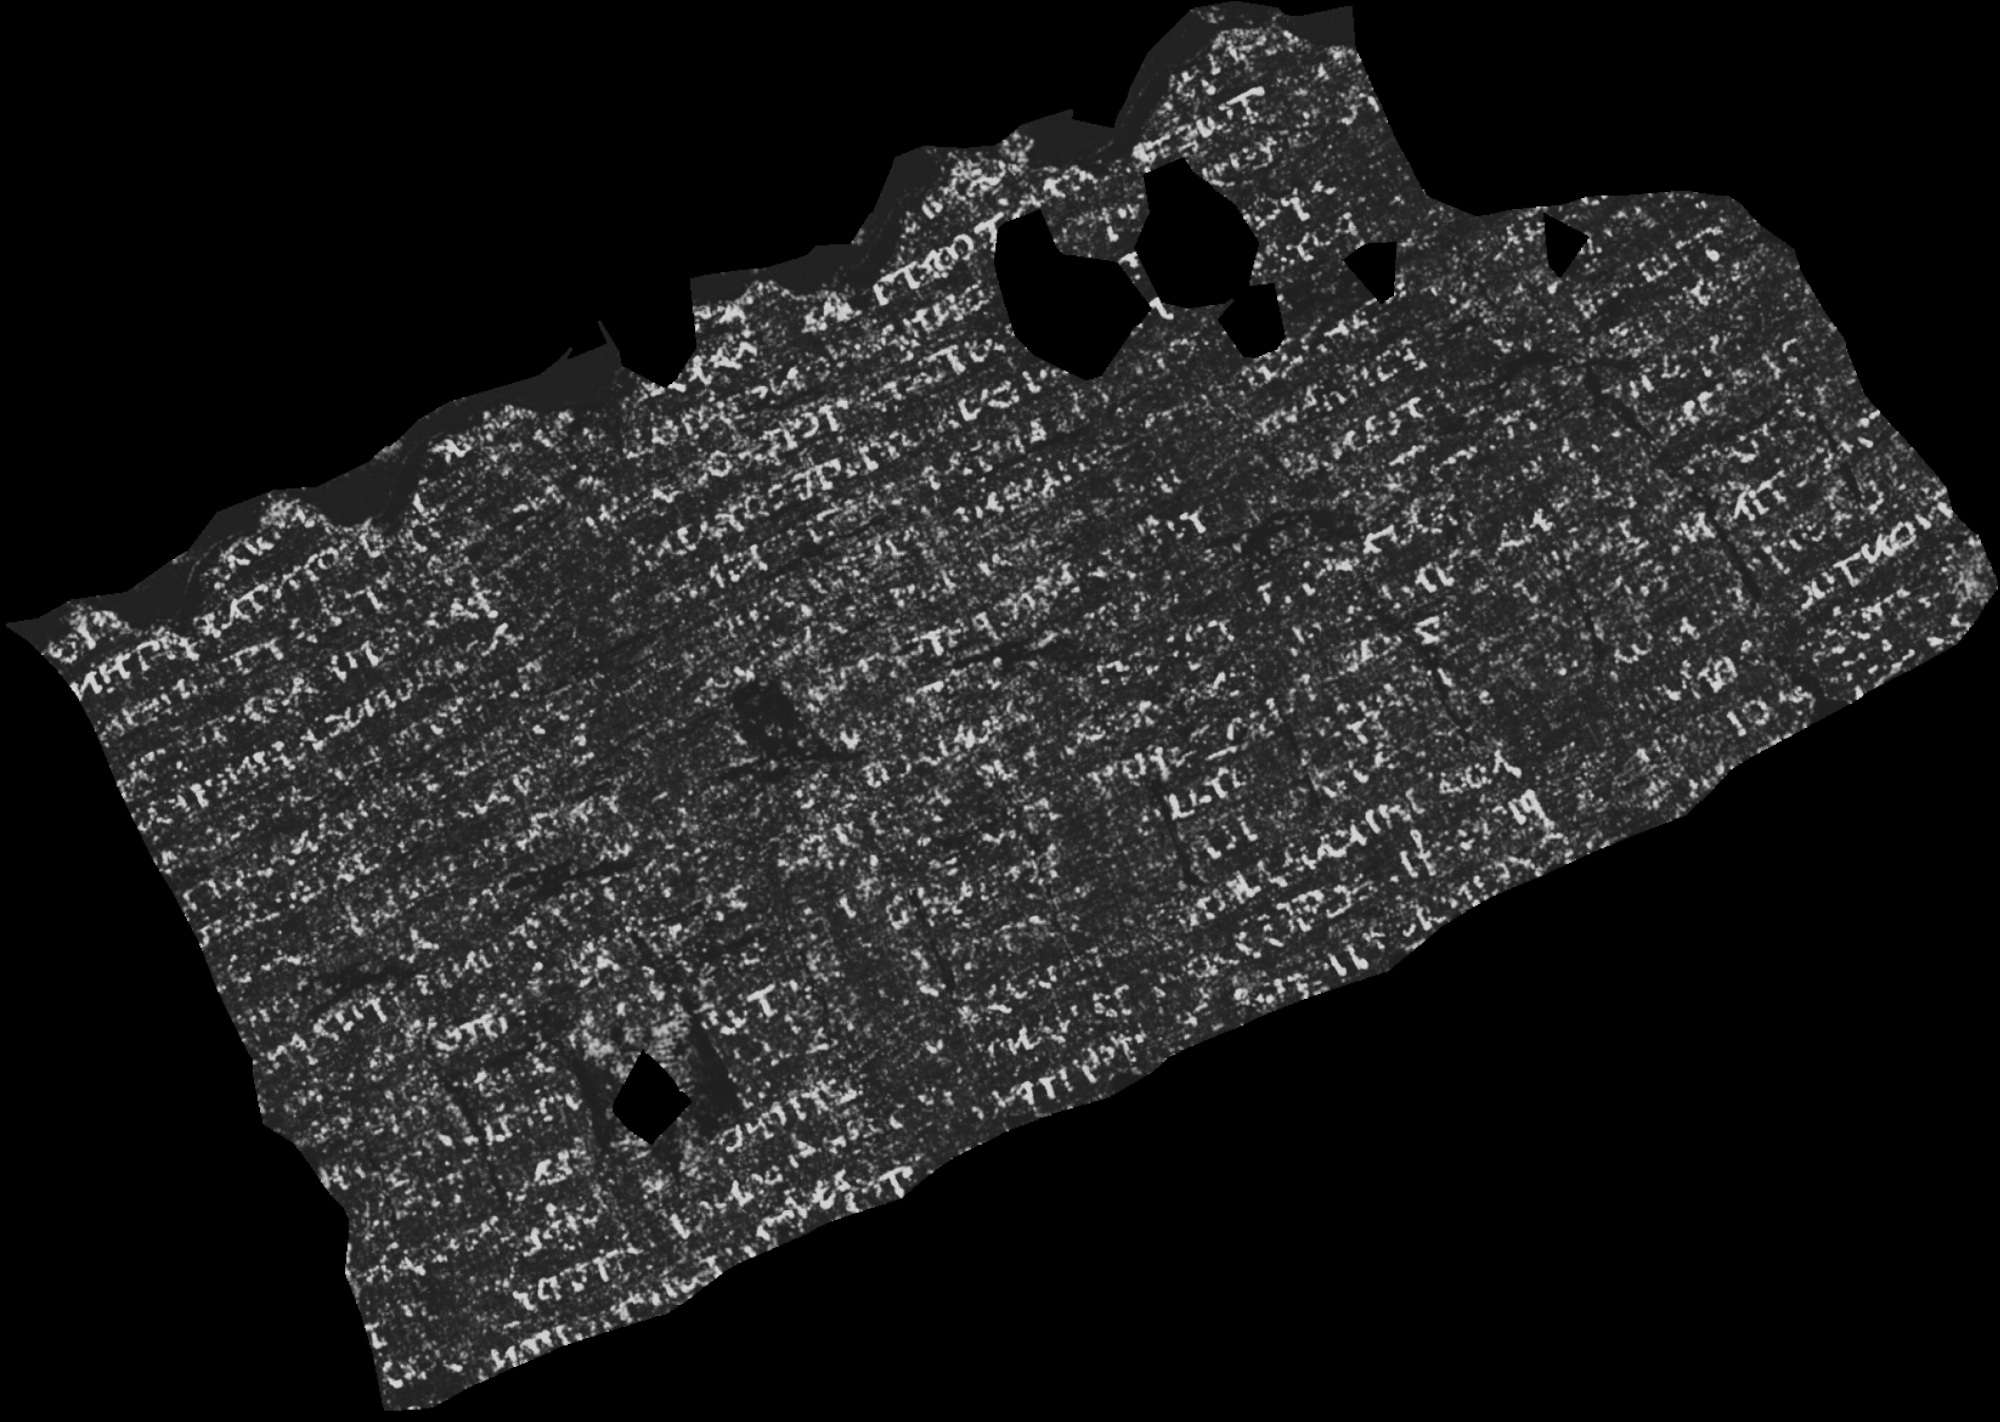
\includegraphics[width=0.8\columnwidth]{predictions_scroll1_thaumato.jpg} 
\caption{Winning Ink Detection Model Predictions for a ThaumatoAnakalyptor Segment in Scroll 1.}
\label{prediction}
\end{figure}


\section{Roadmap}
ThaumatoAnakalyptor should become the go-to tool to unroll ct scans of charred scrolls. Therefore, the pipeline is expected to be improved this year. 
Possible areas of improvements to ThaumatoAnakalyptor from highest to lowest priority to achieve a 90\% readability of each scroll by the end of this year:
\begin{itemize}  
\item Keeping the documentation up-to-date and correcting wrong information, so that everyone has a good time working on the challenge. Ideas: make the mathematical formulations more sound, cross check the documented information and adding references to the exact parts of the code, spelling, make the documentation more understandable, answer other peoples questions in Discord and add them in a FAQ here ...
\item Random\_Walks.py: find another method/improve random walks (for example better starting point sampling strategy which would make the algorithm converge faster, implement concurrent random walks) to reconstruct the sheets from the sheet patches connection graph. Algorithmic suggestions, entirely change the approach to solving the problem with those methods: Variational Shape Analysis, Optimal Transport Theory, Viterbi Algorithm, finding and suggesting new ones, ...
\item Flattening (Jordi already did some amazing work in this regards). Improve flatboi, generate meshes that can be flattened by ABF++, ...
\item Implement performance and integrity tests. Every little test, be it for a function, a pipeline step or the complete ThaumatoAnakalyptor is welcome!
\item Find bugs, fix bugs. Known bugs: Verso and recto naming swapped, Starting point that needs to be on the bottom side of the scroll, flattening often fails close to the scroll center, add your found bugs here, ... 
\item Tuning of the PointCloud extraction technique. Extraction in volume regions where the sheets are completely compressed.
\item Tuning and finding better similarity score functions to compare overlapping sheet patches to build the sheet patches connection graph.
\item In the GUI, implement displaying of the segmented surface points on the 2D slice image (setup already done).
\item Implement capability to add surface patches manually to a running segmentation with the GUI.
\item Improve 3D PointCloud instance segmentation model by adding more training data. Different Scrolls, Fragments, PointCloud extraction techniques, different synthetic data generation.
\item Utilize manual segmentations to generate training data and train on partially annotated subvolumes.
\item Increase instance segmentation subvolume size (from 200x200x200 to maybe 500x500x500?). Devise strategy to generate training data for the increased subvolume.
\item Have the precomputation run on multiple GPU's + test it on such systems (partially implemented). Improve precomputation performance. Inference of the 3D instance segmentation model on multiple GPUs.
\item Improve the mesh reconstruction. Extract high quality meshes that are locally flat, make the mesh manifold, uniform vertex density in the mesh.
\item Improve segmentation trough postprocessing. For example using Brent Olsen's fibre following code to better flatten sheets in the surface volume z dimension.
\item Improve the cylindrical unrolling, add support for unrolling meshes with multiple unconnected surfaces.
\item Analyze different 3D instance segmentation models performances. Does additional data improve instance segmentation (ink predictions, brightness of the voxels belonging to the points, ...)?
\item Identify possible improvements.
\item Tune ink detection. Example: Generate inklabels on segments from ThaumatoAnakalyptor.
\item Detect the papyrus fold close to the scroll center, enabling segmentation over the fold. Adjust mesh reconstruction and cylindrical unrolling to work with segmentations that go over the fold.
\item Performance improvements.
\item Analyze how well the ink detection works with segments produced by ThaumatoAnakalyptor. 
\item Fully automate the generation of the umbilicus.
\item Integrating ppm generation into the pipeline.
\item Add ink detection to the GUI.
\item Improve PointCloud sheet normal estimation for extremely warped papyrus, where the local normal points away from the umbilicus center.
\item Add support for bendy umbilici (non-strictly increasing $Z$ values in the umbilicus.txt).
\item Automate the execution of each processing step.
\end{itemize}

With these improvements, I feel very confident that we will be able to read complete scrolls this year. Let's make history!


\appendices
\section{FAQ} \label{App:FAQ}
\subsection{Where can i put frequently asked questions?}
Here!

\begin{thebibliography}{1}
% Here are a few examples of different citations 
% Article from database
\bibitem{thaumato}J.~Schilliger, ``ThaumatoAnakalyptor'' \emph{GitHub}, Vesuvius Challenge 2023. \url{https://github.com/schillij95/ThaumatoAnakalyptor}. Accessed on: Feb.~15, 2024.
\bibitem{mask3d} % Note the label in the curly brackets. Use the cite the source; e.g., \cite{kopka_latex}
J.~Schult, F.~Engelmann, A.~Hermans, O.~Litany, S.~Tang, B.~Leibe, \emph{Mask3D: Mask Transformer for 3D Semantic Instance Segmentation}, International Conference on Robotics and Automation (ICRA), 2023.


\end{thebibliography}

% This is a hand-made bibliography. If you want to use a BibTeX file, you're on your own ;-)






\end{document}


